\subsection{Joint Alignment Baselines and Fresh Confirmation}\label{app:alignment_confirmation}

Jointly learning a backward map is an established approach to compatibility.
BC-Aligner~\citep{hu2022backward} provides this baseline, while model
stitching~\citep{bansal2021stitching,mai2026stitching} studies related
representation interfaces. We compare alignment targets under a matched
parameterization before testing the HAR construction on new training seeds.
The fixed protocol and development choices were publicly committed before
the corresponding numerical runs.

Development reuses the healthy checkpoints, Adam moments, splits and future
minibatches of seeds $800$--$802$. Both new families learn a bias-free
$64\times64$ map $M$, initialized to identity. Feature alignment minimizes
$\|Mh-h_0\|^2/64$ per example; logit alignment minimizes
$\|AMh+B-z_0\|^2/n_c$. The former is the single-update linear objective of
BC-Aligner with an explicit width normalization, so its coefficient in the
per-example squared-norm convention is $\lambda/64$. There is no historical
composition in this experiment. The two maps share $4{,}096$ trainable
parameters; serving composes $AM$ into one legacy head. The direct head is the
original logit-distillation arm, with $390$ parameters on HAR.

Feature coefficients are $\{0.01,0.1,1,10,100\}$ and logit coefficients are
$\{0.1,1,10\}$. Each family selects the smallest coefficient whose mean
validation disagreement is at most $5\%$, or the largest if none qualifies.
Utility is checked only after this choice. A third candidate applies the fixed
training-only OLS fit to the original protected features and casts the reader
to float32. Table~\ref{tab:alignment_development} includes every candidate.

\begin{table}[htbp]
\centering
\caption{Complete fixed development grid, three seeds per corpus. Primary differences are percentage points relative to detachment; MSE is auxiliary error relative to detachment. Means use validation only. A dagger marks the coefficient selected by mean disagreement before utility is checked; all other coefficients remain visible.}
\label{tab:alignment_development}
\footnotesize
\begin{tabular}{llrrrr}
\toprule
Corpus & target / reader & $\lambda$ & primary & MSE / D & changed \\
\midrule
HAR & Feature map & $0.01^{\dagger}$ & $-0.63$ & $0.728$ & $3.02\%$ \\
HAR & Feature map & $0.1$ & $-0.45$ & $0.733$ & $2.38\%$ \\
HAR & Feature map & $1$ & $-0.09$ & $0.715$ & $1.29\%$ \\
HAR & Feature map & $10$ & $-0.16$ & $0.798$ & $0.79\%$ \\
HAR & Feature map & $100$ & $-0.05$ & $0.941$ & $0.11\%$ \\
HAR & Logit map & $0.1^{\dagger}$ & $-0.18$ & $0.701$ & $0.93\%$ \\
HAR & Logit map & $1$ & $+0.02$ & $0.783$ & $0.45\%$ \\
HAR & Logit map & $10$ & $+0.09$ & $0.942$ & $0.20\%$ \\
HAR & Direct + OLS-fp32 & $0.1^{\dagger}$ & $-0.09$ & $0.703$ & $0.95\%$ \\
\midrule
SNR & Feature map & $0.01$ & $+1.30$ & $0.783$ & $43.17\%$ \\
SNR & Feature map & $0.1$ & $+1.16$ & $0.765$ & $43.72\%$ \\
SNR & Feature map & $1$ & $+1.28$ & $0.785$ & $41.30\%$ \\
SNR & Feature map & $10$ & $+1.24$ & $0.787$ & $31.41\%$ \\
SNR & Feature map & $100^{\dagger}$ & $+0.06$ & $0.807$ & $16.48\%$ \\
SNR & Logit map & $0.1$ & $+1.30$ & $0.768$ & $34.43\%$ \\
SNR & Logit map & $1$ & $+0.09$ & $0.814$ & $15.53\%$ \\
SNR & Logit map & $10^{\dagger}$ & $-0.62$ & $0.880$ & $4.98\%$ \\
SNR & Direct + OLS-fp32 & $10^{\dagger}$ & $-0.65$ & $0.880$ & $3.63\%$ \\
\bottomrule
\end{tabular}
\end{table}


On HAR, feature alignment selects $0.01$ and loses $0.63$ primary points,
missing the half-point utility gate. Stronger feature penalties have viable
validation tradeoffs: at $\lambda=1$, primary changes by $-0.09$ points, MSE
is $0.715$ of detachment, and disagreement is $1.29\%$. Thus the compatibility-only selection policy misses a viable
feature-alignment tradeoff. Logit-map $0.1$ and the direct-head OLS fit pass and open HAR
confirmation. On SNR, feature-map $100$ still changes $16.5\%$ of decisions;
logit-map $10$ and direct-head OLS lose $0.62$ and $0.65$ primary points.
None opens confirmation, and no coefficient is retuned.

We train ten new HAR seeds, $1300$--$1309$, on the same official train/test
benchmark, with new healthy checkpoints and the fixed low-label reconstruction
recipe. Detached, joint and direct-head branches are paired with the selected
logit map; OLS changes only the final reader on the direct-head features.
The bank allocates $\delta=0.05/160$ per consumer, covering up to two corpora,
ten seeds, four protected readers and two monitor sizes. Unused allocations
are retained. The primary monitor has $1{,}024$ uniform inputs. A nested
$2{,}048$-input monitor reports additional observation cost and cannot replace
a failed primary decision.

\begin{table}[htbp]
\centering
\caption{Fresh HAR confirmation, seeds $1300$--$1309$. Primary values are absolute accuracy for detachment and paired percentage-point differences for other rows; brackets are $95\%$ intervals. MSE is reconstruction error relative to detachment. Certified counts use the primary $1{,}024$-input monitor and fixed $160$-consumer tail allocation. Native float32 CPU ratios return both current and legacy outputs at batch $1{,}024$. OLS changes only the reader.}
\label{tab:alignment_confirmation}
\footnotesize
\setlength{\tabcolsep}{4pt}
\begin{tabular}{lrrrrr}
\toprule
Arm & primary & MSE / D & changed & certified & CPU \\
\midrule
Detach & $0.909$ & $1.000$ & $3.71\%$ & --- & --- \\
Joint & $+0.02\ [-0.38,+0.43]$ & $0.767$ & $27.66\%$ & --- & --- \\
Direct & $+0.30\ [-0.01,+0.61]$ & $0.780$ & $1.67\%$ & $10/10$ & $1.064\times$ \\
Logit map & $+0.42\ [+0.03,+0.80]$ & $0.777$ & $1.64\%$ & $9/10$ & $1.067\times$ \\
OLS-fp32 & $+0.30\ [-0.01,+0.61]$ & $0.780$ & $1.46\%$ & $10/10$ & $1.071\times$ \\
\bottomrule
\end{tabular}
\end{table}


The direct head meets the complete confirmation criterion. Reconstruction MSE
is $\FreshMse$ of detachment, with paired $95\%$ interval
$[\FreshMseLow,\FreshMseHigh]$, and primary accuracy differs by
$+\FreshGain$ points $[\FreshGainLow,\FreshGainHigh]$. This interval clears
the $-0.5$-point noninferiority margin. Mean legacy disagreement is
$\FreshDirectChanged\%$, and all ten primary-monitor bounds meet the
five-point budget. OLS reduces disagreement to $\FreshOlsChanged\%$ with
the same primary and reconstruction outcomes and ten certificates. The
logit map has $1.64\%$ mean disagreement but certifies nine seeds. Its ten
secondary-monitor certificates leave that primary failure unchanged.

\begin{figure}[H]
\centering
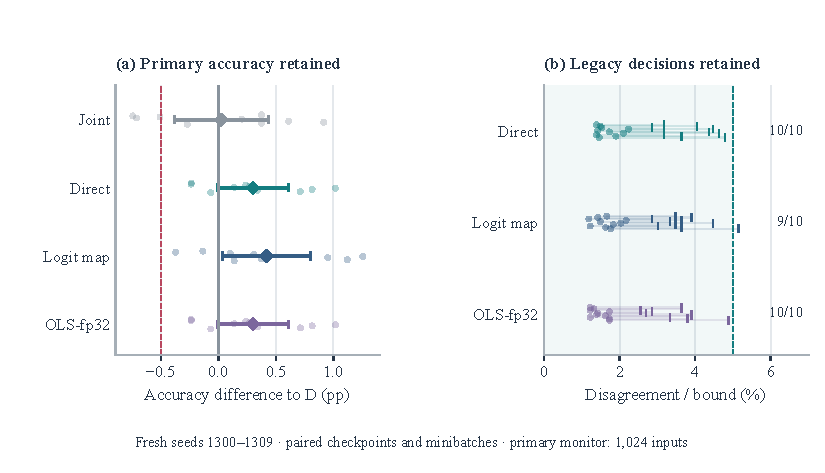
\includegraphics[width=\linewidth]{figures/fig_alignment_confirmation.pdf}
\caption{Fresh HAR confirmation separates aggregate utility from individual
consumer acceptance. (a) All ten paired primary differences, their means and
$95\%$ intervals; the dashed line is the $-0.5$-point margin. (b) Each seed's
observed legacy disagreement (dot) and finite-population upper bound (tick),
with certificate counts at the fixed $5\%$ budget. Direct and OLS-fp32 share
the same encoder, current head and auxiliary head. These are new training
seeds; the earlier $9/10$ HAR study and retrospective audit remain separate.}
\label{fig:alignment_confirmation}
\end{figure}

An isolated serving audit evaluates both heads in float32, using four CPU
threads, five warm-ups and $51$ alternating repetitions. At batch $1{,}024$,
direct and OLS ratios are $\FreshDirectLatency\times$ and
$\FreshOlsLatency\times$ current-only inference; at batch one they are
$\FreshDirectSingleLatency\times$ and $\FreshOlsSingleLatency\times$.
Both outputs use one encoder call. The additional reader occupies $390$
float32 parameters ($1{,}560$ bytes). Both arms also meet the original
diagnostic timing limits, whose current head computes logits in float64.
Native primary predictions match that diagnostic across all $50$ saved
branch endpoints.

Independent tensor replay reproduces all $50$ metric sets and the protected
readers' bounds exactly, including the OLS fitting conditions. Casting OLS
to float32 changes $11$ seed--example predictions among $29{,}470$ comparisons
with its float64 fit, with maximum logit difference $0.182$; all reported OLS
certificates evaluate the actual float32 reader. The fresh HAR confirmation therefore retains a bounded fraction of legacy
decisions under the actual float32 implementation.
